\chapter{Hypergraphen}
\label{chpt:hypergraphs}

\begin{definition}[Hypergraph]
    Ein Hypergraph $ H = (V, E) $ ist ein Tupel aus einer Knotenmenge $ V $ und einer Kantenmenge $ E \subseteq 2^V $ mit $ \emptyset \notin E $.
\end{definition}

\begin{definition}[Einfach]
    Ein Hypergraph $ H = (V, E) $ ist \textit{einfach}, falls für $ e, f \in E $ gilt, dass $ e \subseteq f \Rightarrow e = f $.
\end{definition}

\begin{definition}[Kantenzug/Weg/Pfad]
    Sei $ H $ ein Hypergraph.
    Ein Kantenzug ist eine Folge $ (x_0, e_1, x_1, e_2, \dots, e_n, x_n) $ mit $ x_i \in V $ und $ e_i \in E $ und $ x_{i - 1}, x_i \in e $.
\end{definition}

\begin{definition}[Minimaler Pfad]
    Ein \textit{minimaler Pfad} in einem Hypergraphen ist ein Kantenzug $ (x_0, e_1, \dots, e_n, x_n) $ mit $ e_i \cap e_j \ne \emptyset $ gdw. $ j = i + 1 $.
\end{definition}

\begin{lemma}
    Jeder Kantenzug enthält einen minimalen Pfad.
\end{lemma}

\begin{proof}
    Sei $ K = (x_0, e_1, \dots, e_n, x_n) $ ein Kantenzug und nicht minimal.
    Dann ex. zwei Kanten $ e_i $ und $ e_j $ mit $ e_i \cap e_j \ne \emptyset $ und $ j \ne i + 1 $.
    Sei $ y \in e_i \cap e_j $.
    Reduziere:
    \begin{align*}
        K = e_0 x_1 e_1 \dots x_i e_i & \underbrace{x_{i + 1} \dots x_j}_{\text{reduziere zu } y} e_j \dots x_n e_n \\
        K' = e_0 x_1 e_1 \dots x_i e_i & y e_j \dots x_n e_n
    \end{align*}

    Nun ist $ K' $ minimal bzgl. $ e_i $ und $ e_j $.
    Falls $ K' $ aber weiterhin nicht minimal, iteriere Reduktion.
\end{proof}

\begin{remark}
    Minimale Kantenzüge sind i.~A. nicht eindeutig.
\end{remark}

\begin{definition}[Sub-Hypergraph]
    Sei $ H = (V, E) $ ein Hypergraph.
    $ H' = (V', E') $ ist ein Sub-Hypergraph, falls:
    \begin{enumerate}
        \item $ V' \subseteq V $,
        \item $ E' \subseteq E $ und
        \item $ \forall e \in E': e \subseteq V' $.
    \end{enumerate}
\end{definition}

\begin{definition}[Induzierter Sub-Hypergraph]
    Sei $ H = (V, E) $ ein Hypergraph.
    $ H' = (V', E') $ ist der von $ V' \subseteq V $ induzierte Sub-Hypergraph, falls $ E' = \{ e \in E \mid e \subseteq V' \} $.
\end{definition}

\begin{definition}[Partieller Hypergraph]
    Sei $ H = (V, E) $ ein partieller Hypergraph.
    $ H' = (V', E') $ ist ein partieller Hypergraph von $ H $, falls:
    \begin{enumerate}
        \item $ V' \subseteq V $ und
        \item $ E' \subseteq \{ e \cap V' \mid e \in E \} $.
    \end{enumerate}
\end{definition}

\begin{definition}[Cut vertex]
    Sei $ H = (V, E) $ ein Hypergraph.
    $ v \in V $ ist ein \textit{schwacher cut vertex}, falls für $ H' = (V', E') $ mit:
    \begin{enumerate}
        \item $ V' \subseteq V $ und
        \item $ E' = \{ e \setminus \{ v \} \mid e \in E \} $,
    \end{enumerate}
    $ H' $ mehr Zusammenhangskomponenten hat als $ H $.

    $ v $ ist ein \textit{starker cut vertex}, falls für $ H' $ gilt:
    \begin{enumerate}
        \item $ V' = V \setminus \{ v \} $ und
        \item $ E' = \{ e \in E \mid x \notin e \} $,
    \end{enumerate}
    und $ H' $ bzgl. dieser Bedingungen mehr Zusammenhangskomponenten hat als $ H $.
\end{definition}

\begin{definition}[König-Graph]
    Sei $ H = (V_H, E_H) $ ein Hypergraph.
    $ G = (V, E) $ ist der \textit{König-Graph} zu $ H $, falls:
    \begin{enumerate}
        \item $ V = V_H \cup E_H $ und
        \item $ E = \{ \{ x, e \} \mid x \in V_H, e \in E_H \} $.
    \end{enumerate}
\end{definition}

\begin{remark}
    Jeder König-Graph ist bipartit.
\end{remark}

\begin{lemma}
    Ein Hypergraph ist zusammenhängend, falls der König-Graph zusammenhängend ist.
\end{lemma}

\begin{definition}[Dualer Hypergraph]
    Sei $ H = (V, E) $ ein Hypergraph.
    Der duale Hypergraph $ \bar H $ zu $ H $ ergibt sich aus der Interpretation der Kanten-Knoten im König-Graph $ G $ zu $ H $ als Knoten-Knoten und der Knoten-Knoten als Kanten-Knoten.
\end{definition}

\begin{remark}
    Der duale Hypergraph existiert nur, falls es keine isolierten Knoten im Hypergraphen gibt.
    Diese würde die leere Kantenmenge induzieren.
\end{remark}

\begin{definition}[Separiert]
    Ein Hypergraph $ H = (V, E) $ ist \textit{separiert}, falls gilt:
    \begin{equation*}
        \forall v, w \in V \exists e \in E: (v \in e \land w \notin e) \lor (w \in e \land v \notin e)
    \end{equation*}
\end{definition}

\section{Gerichtete Hypergraphen}

\begin{definition}[Gerichteter Hypergraph]
    Ein \textit{gerichteter Hypergraph} $ H = (V, E) $ ist ein Tupel aus einer Knotenmenge $ V $ und einer Kantenmenge $ E \subseteq 2^V \times 2^V $.
    Wir schreiben $ e^- $ für die erste Komponente einer Kante $ e \in E $ und $ e^+ $ für die zweite Komponente.

    Für $ e \in E $ kann $ e^- \cap e^+ = \emptyset $ gefordert werden.
\end{definition}

\begin{definition}[Kantenzug]
    Sei $ H = (V, E) $ ein gerichteter Hypergraph.
    Eine Folge $ K = (x_0, e_1, x_1, e_2, \dots, e_n, x_n) $ ist ein Kantenzug, falls $ x_i \in e_{i + 1}^- $ und $ x_i \in e_i^+ $.
\end{definition}

\begin{definition}[Minimaler Kantenzug]
    Ein Kantenzug $ K = (x_0, e_1, x_1, e_2, \dots, e_n, x_n) $ ist \textit{minimal}, falls $ e_i^+ \cap e_j^+ \ne \emptyset $ gdw. $ j = i + 1 $ und $ x_0 \in e_i^- $ gdw. $ i = 1 $ und $ x_n \in e_i^+ $ gdw. $ i = n $.
\end{definition}

\begin{definition}[B-Hypergraph]
    Ein gerichteter Hypergraph $ H = (V, E) $ ist ein \textit{B-Hypergraph}, falls für $ e \in E $ $ |e^+| = 1 $ gilt.
\end{definition}

\begin{remark}
    Für gerichtete Hypergraphen kann der König-Graph entsprechend mit gerichteten Kanten definiert werden.
\end{remark}

\section{Inzidenzstrukturen für Hypergraphen}

\begin{definition}[Inzidenzmatrix]
    Sei $ H = (V = \{ v_1, \dots, v_n \}, E = \{ e_1, \dots, e_n \}) $ ein Hypergraph.
    $ I \subseteq \{ 0, 1 \}^{n \times m} $ ist die Inzidenzmatrix zu $ H $, falls:
    \begin{multicols}{2}
        Für ungerichtete Hypergraphen:
        \begin{equation*}
            I_{kl} = \begin{cases}
                1, & x_k \in e_l \\
                0, & x_k \notin e_l
            \end{cases}
        \end{equation*}
        \columnbreak

        Für ungerichtete Hypergraphen:
        \begin{equation*}
            I_{kl} = \begin{cases}
                +1, & x_k \in e_l^+ \\
                -1, & x_k \in e_l^- \\
                0, & \text{sonst}
            \end{cases}
        \end{equation*}

        Im gerichteten Fall ist die Inzidenzmatrix nur definiert, falls für $ e \in E $ $ e^- \cap e^+ = \emptyset $ gilt.
    \end{multicols}
\end{definition}

\begin{proposition}
    Sei $ I $ die Inzidenzmatrix eines ungerichteten Hypergraphen $ H = (V, E) $ und $ A $ die Adjazenzmatrix des König-Graphen zu $ H $.
    Dann gilt:
    \begin{equation*}
        A = \begin{bmatrix}
            0^{V \times V} & I \\
            I^\top & 0^{E \times E}
        \end{bmatrix}
    \end{equation*}
\end{proposition}

\section{Anwendung von Hypergraphen}

Ein System von chemischen Reaktionen kann durch einen gewichteten und gerichteten Hypergraphen $ H = (V, E, w) $ beschrieben werden.
Ein Knoten $ v \in V $ stellt ein chemisches Element dar; dies kann eine der Funktionen: Futter des System, Zwischenprodukt oder Endprodukt einnehmen.
Eine Kante $ e \in E $ stellt eine chemische Reaktion dar.
$ e^- $ sind die Stoffe, die in der Reaktion verbraucht werden, $ e^+ $ die Stoffe, die erzeugt werden.
Kanten mit $ e^- = \emptyset $ können genutzt werden, um den Zufluss von Produkten aus dem System zu modellieren, Kanten mit $ e^+ = \emptyset $ um den Abfluss zu modellieren.
$ w : E \times V \to \nats $ stellt den Verbrauch eines Element bzw. Generierung eines Produkts in einer spezifischen Reaktion dar.
Diese Funktion bildet Elemente, die nicht an einer Reaktion teilnehmen auf $ 0 $ ab.

\begin{definition}[Stoichiometrische Koeffzienten/Matrix]
    Die stoichiometrische Matrix $ S_H $ eines gewichtete, gerichteten Reaktions-Hypergraphen $ H = (V, E, w) $ ist die Inzidenzmatrix zu $ H $ komponentenweise multipliziert mit $ w $.
\end{definition}

\begin{remark}
    Im Allgemeinen hat eine entrspechende stoichemetrische Matrix die in Abbildung \ref{fig:stoich} dargestellte Form, wobei $ E $ für die Einheitsmatrix steht.

    In der \textbf{F}lux \textbf{B}alance \textbf{A}nalysis (FBA) bzw. der \textbf{M}ultiple \textbf{F}lux \textbf{A}nalysis (MFA) wird untersucht, wie solche Systeme dargestellt als stoichemetrische Matrix $ S $ mit einem Gewichtungs-Vektor $ v \in \reals^E $, der die Reaktions- bzw. Zu- und Abflussraten darstellt, optimiert werden können.
    Dabei wird die folgende Gleichung betrachtet:
    \begin{equation*}
        S \cdot v = 0
    \end{equation*}

    Fixiert wird dabei einerseits die Matrix, um herauszufinden unter welche Zugabe von Stoffen und unter welcher Reaktionsrate optimal viele Endprodukte erzeugt werden können.
    Andererseits kann auch der Vektor $ v $ fixiert werden, um zu untersuchen, wie das System optimiert werden kann, d.h. welche Reaktionen ggfs. \textit{besser} ablaufen sollten.

    \begin{figure}
        \centering
        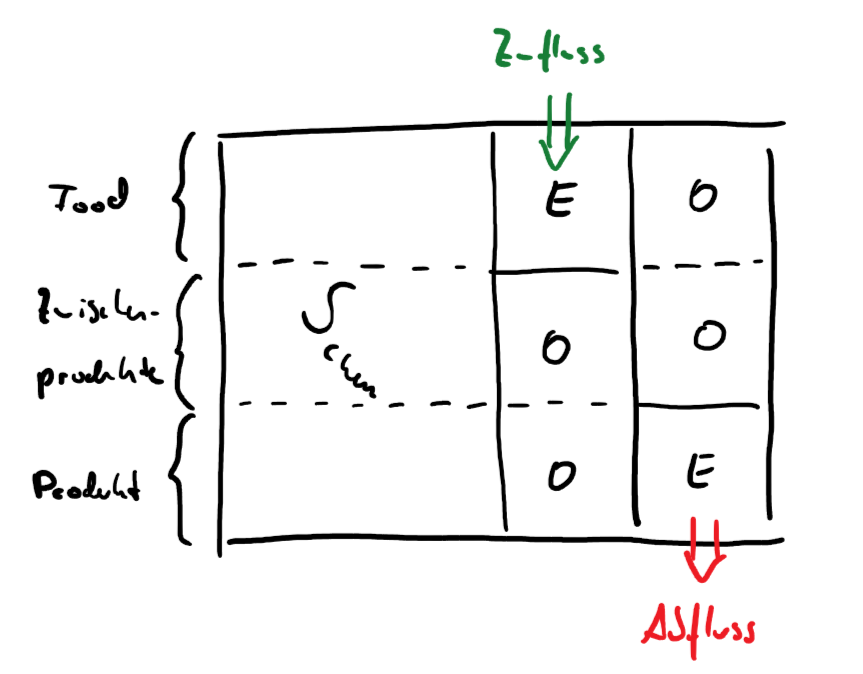
\includegraphics[width=0.75\textwidth]{figures/stoichiometrisch.png}
        \caption{Stoichemetrische Matrix als Reaktions-System}
        \label{fig:stoich}
    \end{figure}
\end{remark}
